\documentclass{article}
\usepackage[UTF8]{ctex}
\usepackage{amsmath}
\usepackage{graphicx}
\usepackage{booktabs}

%要运行该模板,LaTex需要安装CJK库以支持汉字.
%字体大小为12像素,文档类型为article
%如果你要写论文,就用report代替article
%所有LaTex文档开头必须使用这句话
%使用支持汉字的CJK包

%开始CJK环境,只有在这句话之后,你才能使用汉字
%另外,如果在Linux下,请将文件的编码格式设置成GBK
%否则会显示乱码

	%这是文章的标题
	\title{HPC Final Project}
	%这是文章的作者
	\author{12132431 钟昊辰}
	%这是文章的时间
	%如果没有这行将显示当前时间
	%如果不想显示时间则使用 \date{}
	\date{2022/6/9}
	%以上部分叫做"导言区",下面才开始写正文
	\begin{document}
		%先插入标题
		\maketitle     %主要的作用是用于生成标题的作用 content contain \title \author \date
		%再插入目录
		
		\tableofcontents   %主要的作用适用于生成目录的作用

		\clearpage
		
		\section{Problem B :陈述}
		考虑一维(1D)域中的热传导方程$\Omega:=(0,1)$。域的边界为$\Gamma=\{0,1\}$。设$f$为单位体积的热源,$u$ 为温度,它是关于x和t的函数;$\rho$为密度,$c$为热容,$u_0$为初始温度,$\kappa$为传热系数,$n_x$为笛卡尔坐标系下的单位法向量。边界条件为$\Gamma_g$上规定的温度函数$g$和$\Gamma_h$上的热通量函数$h$,它们均为x和t的函数。边界$\Gamma$允许非重叠分解:$ \Gamma = \bar{\Gamma_g \cap \Gamma_h},\emptyset = \Gamma_g \cup \Gamma_h$。热传导方程可以表述如下:
		$$
		\rho c \frac{\partial u}{\partial t}-\kappa\frac{\partial^2 u}{\partial x^2}=f
		\quad on \quad \Omega \times (0,T)
		 $$	
		$$
		u=g
		\quad on \quad \Gamma_g \times (0,T)
		$$
		$$
		\kappa \frac{\partial u}{\partial x}n_x=h
		\quad on \quad \Gamma_h \times (0,T)
		$$
		$$
		u|_{t=0}=u_0
		\quad in \quad \Omega.
		$$
		考虑如下所述的边界条件,初始条件和函数:
		$$ 
		\left\{
		\begin{aligned}
			B.C.s \quad u(0,t)=u(1,t)=0 \\
			I.C. \quad u(x,0)=e^x \\
			f(x,t)=sin(l\pi x) \\
			\kappa=1.0 \\
		\end{aligned}
		\right.
		$$
		其中$l=constant$,令$l=1.0$。\\
		使用有限差分法求解该问题。利用泰勒展开公式,将方程中的偏导数项展开为差分格式的公式。如果一个差分格式每一排各节点上的数值可直接由前面各排节点的数值计算得到,则称为显示差分格式。如果一个差分格式每一排各节点的数值需要求解一个线性代数方程组同时确定,则称为隐式差分格式。在时间上采用后向差分格式,在空间上使用中心差分格式,则热传导方程的显式差分格式可以表示如下:
		$$
		\frac{u^{n+1}_j-u^n_j}{\Delta t}=\frac{\kappa }{\rho  c}\frac{u^{n}_{j+1}-2u^{n}_j+u^{n}_{j-1}}{{\Delta x}^2}+\frac{f}{\rho c}
		$$
		其中$n$为时间步,$j$为空间上的网格点。考虑时间正向积分,将所有时间步为n的项移至右侧,得到
		$$
		u_j^{n+1}=\frac{\kappa \Delta t}{\rho  c \Delta x^2}u^{n}_{j-1}+(1-2\frac{\kappa \Delta t}{\rho  c \Delta x^2})u^{n}_{j}+\frac{\kappa \Delta t}{\rho  c \Delta x^2}u^{n}_{j+1}+\frac{f \Delta t}{\rho c}
		$$
		隐式差分格式的公式
		$$
		\frac{u^{n+1}_j-u^n_j}{\Delta t}=\frac{\kappa }{\rho  c}\frac{u^{n+1}_{j+1}-2u^{n+1}_j+u^{n+1}_{j-1}}{{\Delta x}^2}+\frac{f}{\rho c}
		$$
		同样,其中$n$为时间步,$j$为空间上的网格点。考虑时间正向积分,将所有时间步为$n+1$的项移至左侧,得到
		$$-\frac{\kappa \Delta t}{\rho c {\Delta x}^2}u^{n+1}_{j-1}+(1+2\frac{\kappa \Delta t}{\rho c {\Delta x}^2})u^{n+1}_j-\frac{\kappa \Delta t}{\rho c {\Delta x}^2}u^{n+1}_{j+1}=u^{n}_j+\frac{f\Delta t}{\rho c}
		$$
		令$CFL=\frac{\kappa \Delta t}{\rho  c \Delta x^2}$,在计算流体力学力学中,$CFL$是用来表征数值方程稳定性的变量。在PETSc中,我们需要使用矩阵运算功能来求解上述方程,同时由于$f$与$t$无关,所以将显示差分格式表示为矩阵形式:
		$$
		\begin{aligned}
		\begin{bmatrix}
			u_0^{n+1} \\
			u_1^{n+1} \\
			\vdots \\
			u_j^{n+1} \\
			\vdots \\
			u_{N-1}^{n+1} \\
		\end{bmatrix}
		=
		\begin{bmatrix}
			1-2CFL & CFL & & & & \\
			CFL & 1-2CFL & CFL & & &\\
			 & \ddots &  \ddots & \ddots & &\\
			 & & \ddots & \ddots & \ddots &\\
			 & & & CFL & 1-2CFL & CFL \\
			 & & & & CFL & 1-2CFL\\
		\end{bmatrix}
		\\
		\times
	    \begin{bmatrix}
	    	u_0^n \\
	    	u_1^n \\
	    	\vdots \\
	        u_j^n \\
	    	\vdots \\
	    	u_{N-1}^n \\
	    \end{bmatrix}+
     	\begin{bmatrix}
    		f_0 \\
    		f_1 \\
    		\vdots \\
    		f_j^n \\
    		\vdots \\
    		f_{N-1}^n \\
    	\end{bmatrix}
    	\end{aligned}
		$$
		其中N是网格分辨率,即节点数。同样,将隐式差分格式表示为矩阵形式:
		$$
		\begin{aligned}
		\begin{bmatrix}
			1+2CFL & -CFL & & & & \\
			-CFL & 1+2CFL & -CFL & & &\\
			& \ddots &  \ddots & \ddots & &\\
			& & \ddots & \ddots & \ddots &\\
			& & & -CFL & 1+2CFL & -CFL \\
			& & & & -CFL & 1+2CFL\\
		\end{bmatrix}
		\begin{bmatrix}
			u_0^{n+1} \\
			u_1^{n+1} \\
			\vdots \\
			u_j^{n+1} \\
			\vdots \\
			u_{N-1}^{n+1} \\
		\end{bmatrix}
		\\
		=
		\begin{bmatrix}
			u_0^n \\
			u_1^n \\
			\vdots \\
			u_j^n \\
			\vdots \\
			u_{N-1}^n \\
		\end{bmatrix}+
		\begin{bmatrix}
			f_0 \\
			f_1 \\
			\vdots \\
			f_j^n \\
			\vdots \\
			f_{N-1}^n \\
		\end{bmatrix}
		\end{aligned}
		$$
		由此,我们建构了显示差分和隐式差分的迭代方程。每次迭代过程中,下一时间步的温度向量可以通过当前时间步的温度向量求解。
		
		\clearpage
		
		\section{代码构成}
		
		本节将通过以下几点要求描述代码各部分的功能。\\
		1.主体:代码主要包括3个部分,首先是全局变量,包括网格分辨率N,时间变化率$dt$等,定义在头文件global.h中并赋值;如果需要修改这些参数的值,可以在头文件中修改。第二部分是显式方法求解,位于heat\_transfer\_explicit.c文件中,主要是调用PETSc的函数计算第一章中的显式矩阵表达式,并使用时间步迭代的方式求解温度向量,并且求解了精确解,用于计算误差;第三部分是隐式方法求解,位于heat\_transfer\_implicit.c文件中,主要是调用PETSc的函数计算第一章中的隐式矩阵表达式,并使用时间步迭代的方式求解温度向量,显式和隐式的主要区别是,由于隐式需要同时求解下一时间步的不同位置的所有温度,需要求解一个矩阵方程,因此需要引入头文件petscksp.h,代码的主要结构和显式方法是相同的。
		\\
		2.HDF5:代码实现了使用HDF5进行进程的首次启动,关闭和重启功能。主要方法为:引入一个布尔运算符restart,当restart的值为false时,代码是首次运行,会创建一个HDF5的group,其中有两个dataset,一个用于储存计算出的温度向量$u$,另一个则用于储存参数运行时间,时间变化率,网格分辨率$t,\Delta t,N$,每次迭代都会把以上的参数写入.h5文件。当restart的值为true时,代码是重启状态,会从当前文件夹的.h5文件读入已有的上述参数,并且继续用于计算。并且在之后的每次迭代中,都会把以上的参数写入.h5文件。
		\\测试HDF5功能:分别令终止时间$t_end=1.0,2.0$,令restart=false,运行程序,此时会获得程序运行至时间为1.0和2.0的.h5文件。第二次运行时令restart=true,将$t=1.0$的.h5文件放入文件夹再次运行程序,至$t=2.0$停止。比较两次得到的$t=2.0$的温度数据,如图1所示。可以看到二者完全吻合,说明HDF5代码是有效的。
		\begin{figure}
			\centering
			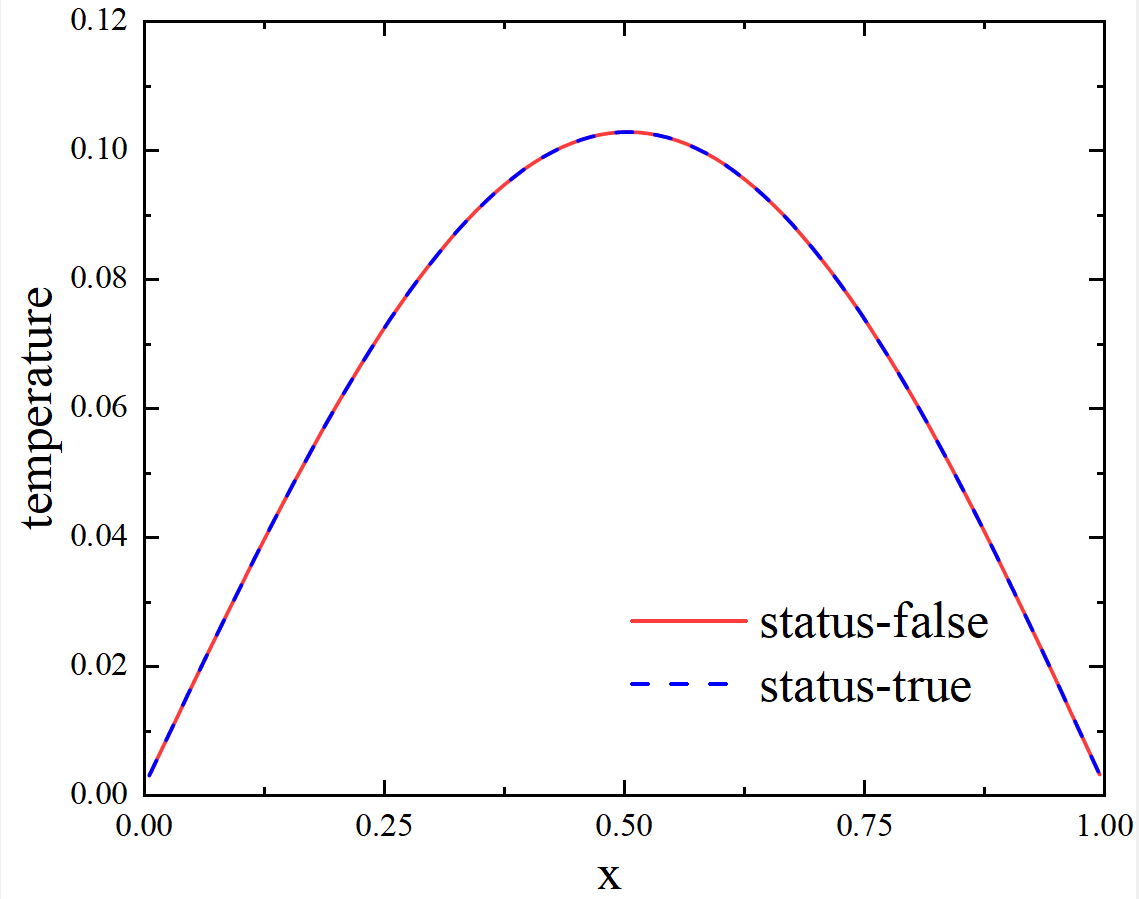
\includegraphics[width=0.7\linewidth]{screenshot001}
			\caption[]{不同状态的程序运行到同一时刻的温度值对比}
			\label{fig:screenshot001}
		\end{figure}
		\\
		3.编程过程中使用了数种防御性编程的方法,如:(1)优化排版,将变量的声明放到了程序开头,并且使用空格优化阅读体验;(2)多次使用PETSc的*View函数检视输出的数值,确保数值稳定或无误;(3)保留了足够数量的注释,用于解释每段函数或者变量的功能;(4)保留了测试用的代码,用于测试代码运行逻辑,等等。
		\\
		4.Makefile:对于显式隐式方法,都有一个对应的Makefile,位于相应文件夹中。可以使用make命令直接编译出可执行文件。(需要将头文件global.h和源文件heat\_transfer\_explicit.c放到同一个文件夹)
		\\
		5.使用Valgrind对程序进行了分析。如图2所示,其中记录了所有函数和内存的调用,耗时比较长的是PETSc的初始化。打开HDF5文件也占用了一定的时间。这个结果是符合预期的,因为程序的主要目的就是反复迭代求解矩阵。
		\begin{figure}
			\centering
			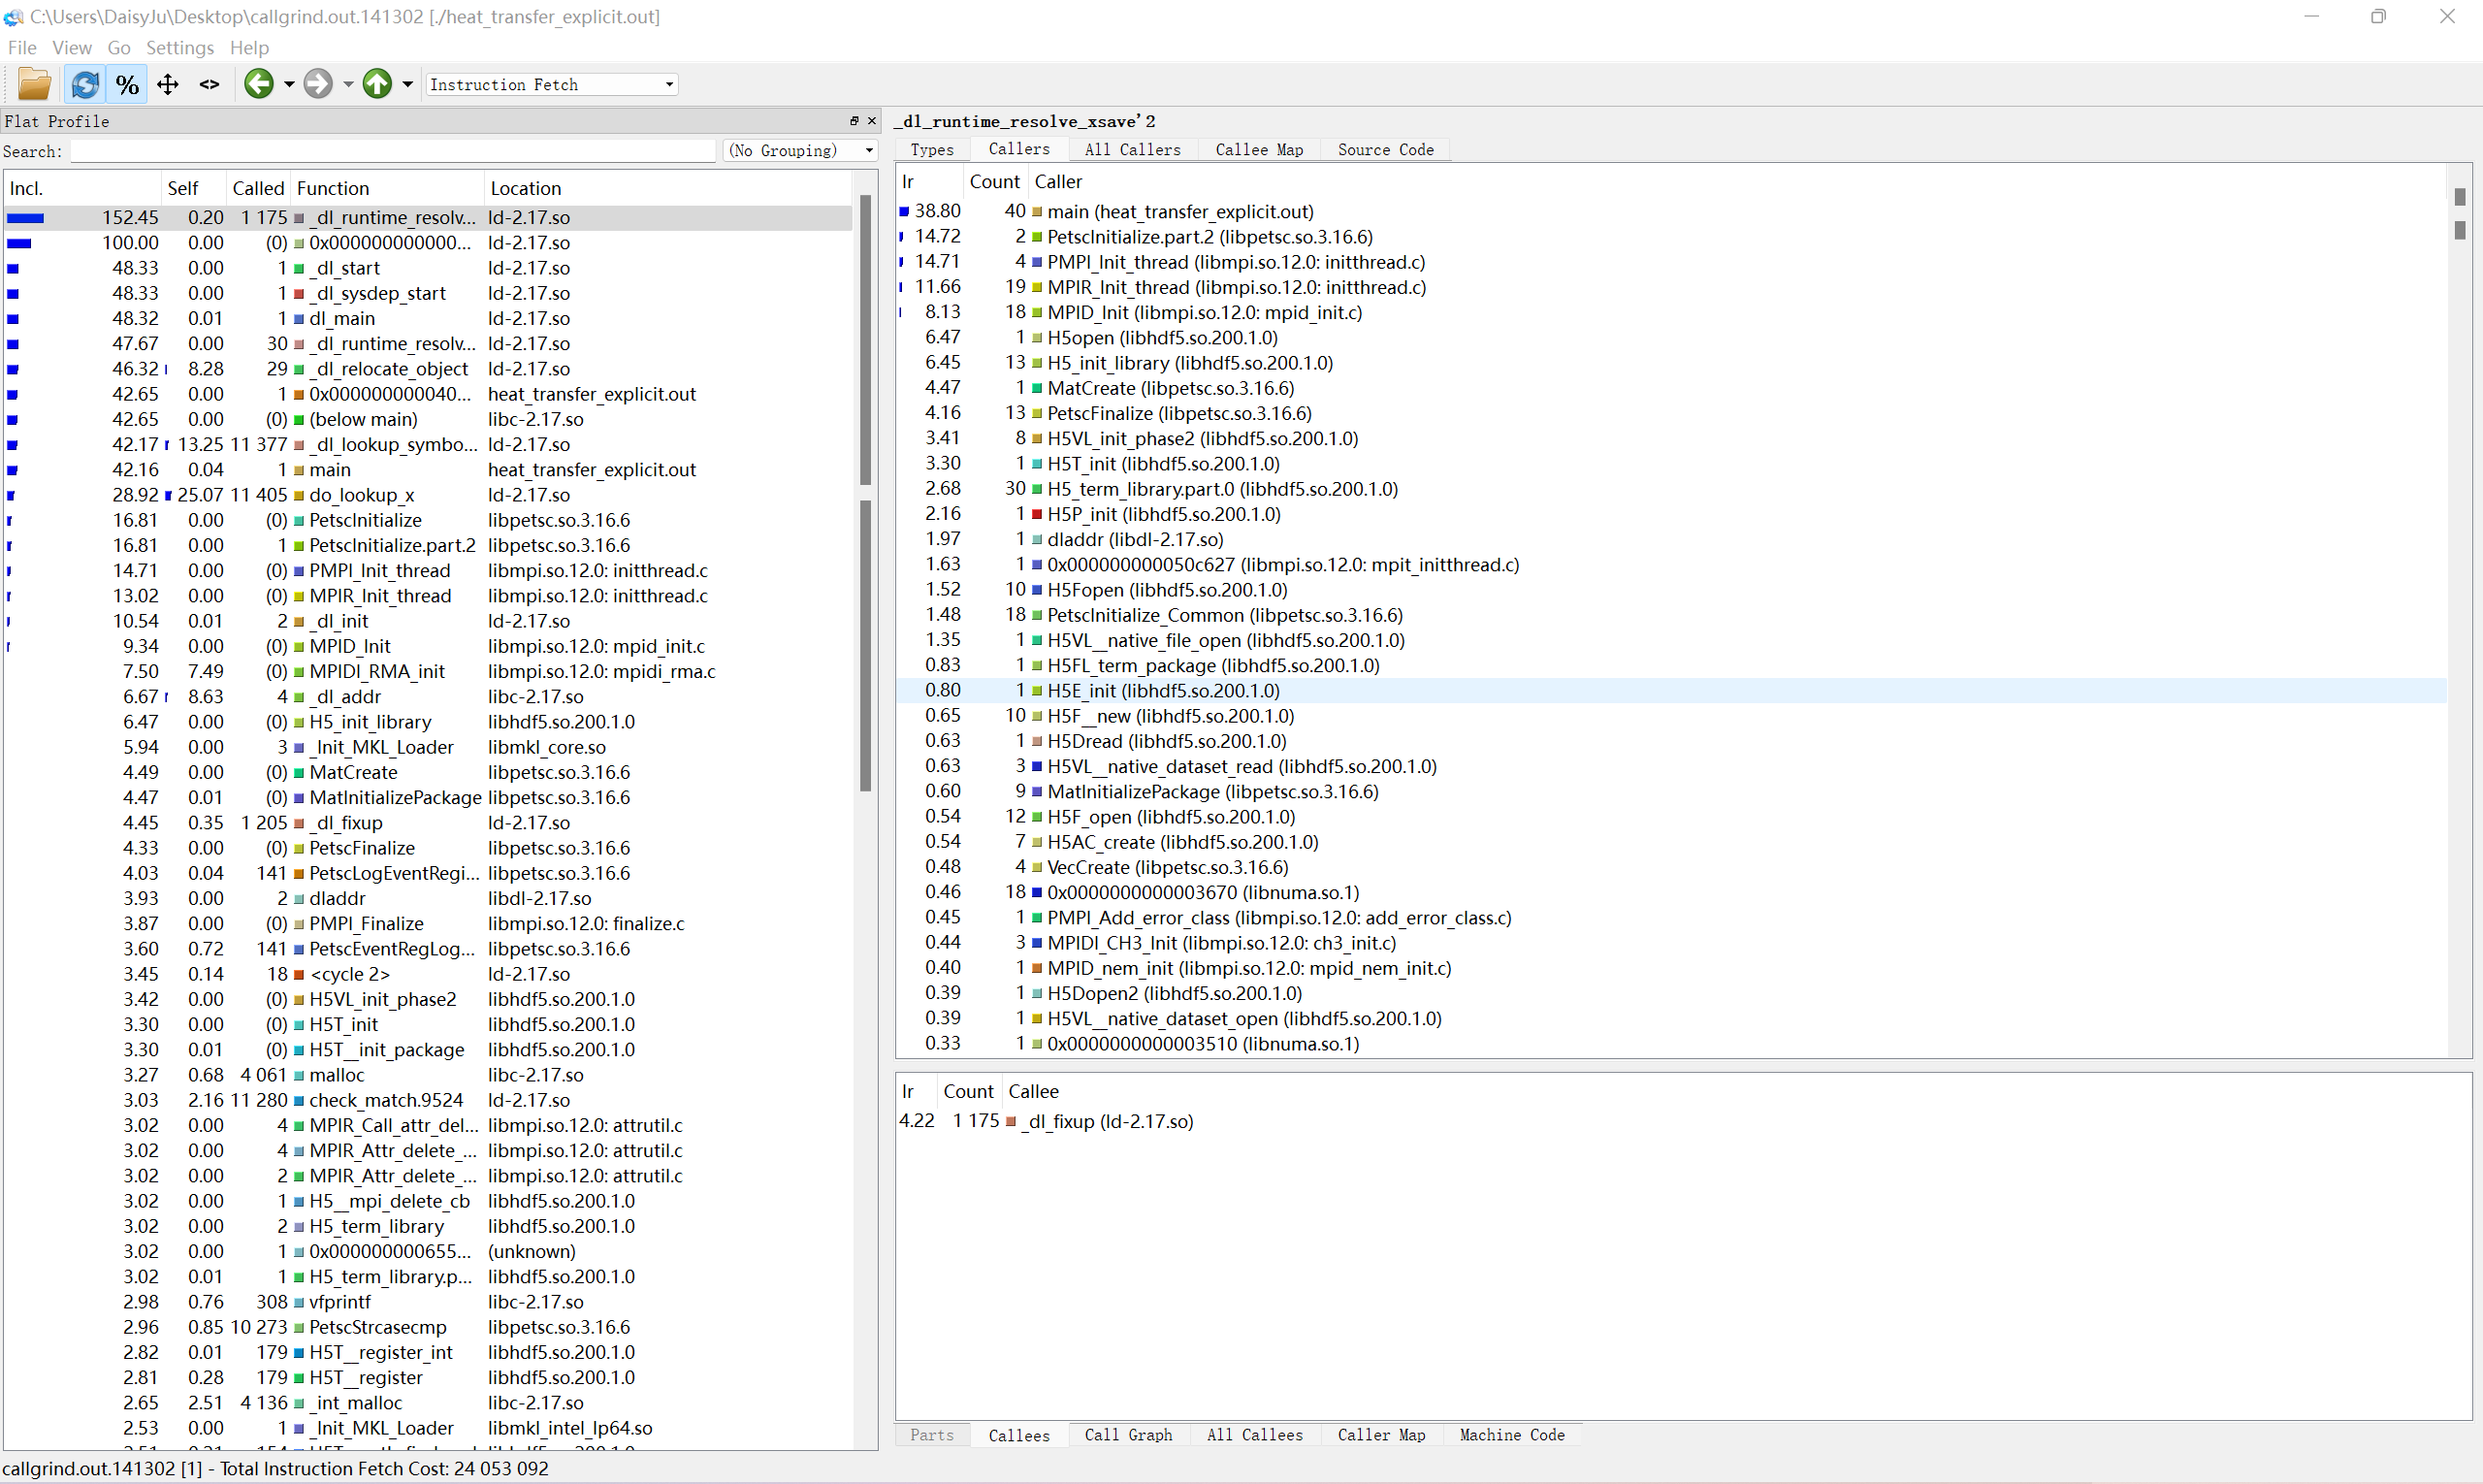
\includegraphics[width=1.0\linewidth]{screenshot002}
			\caption{Kcachegrind程序分析}
			\label{fig:screenshot002}
		\end{figure}
		\\
		6.所有的工作进度都在Github上进行了实时同步。此外所有的测试文件均位于太乙服务器的路径下(先前测试时生成的很多冗余的日志文件都进行了删除):
		\\
		/work/mae-zhonghc/hpc/HPC\_project
		\\
		仓库路径为:
		\\https://github.com/DaisyXiaoJu/HPC\_project
		\\重要说明:本人原与郭琳同学合作二维项目,但是由于后来遇到了难以解决的问题(如解析解求解难度过高),所以后来放弃了二维问题,改为重写一维问题。上面链接是我的个人仓库,原合作仓库地址如下,保存了本人先前的部分工作和commits:
		\\https://github.com/GBoy2509/HPC\_project
		
		\section{代码测试}
		\subsection{方法稳定性}
		在该节中,利用计算流体力学相关知识,使用Von-Neumann's stability analysis(冯诺依曼稳定性分析)方法理论求解方程稳定性。对于显式差分格式:
		$$
		u_j^{n+1}=\frac{\kappa \Delta t}{\rho  c \Delta x^2}u^{n}_{j-1}+(1-2\frac{\kappa \Delta t}{\rho  c \Delta x^2})u^{n}_{j}+\frac{\kappa \Delta t}{\rho  c \Delta x^2}u^{n}_{j+1}+\frac{f \Delta t}{\rho c}
		$$
		它的舍入误差方程表示为:
		$$
		\delta u_j^{n+1}=(1-2CFL)\delta u_j^n + CFL(u^{n}_{j-1}+u^{n}_{j+1})
		$$
		冯诺依曼稳定性分析的流程如下,其中使用了欧拉公式:
		$$
		\delta u_j^n \sim e^{\sigma t^n}\cdot e^{i(k\cdot x_j)} \sim e^{\sigma n\Delta t}\cdot e^{i(kj\Delta x)}
		$$
		$$
		e^{\sigma (n+1)\Delta t}\cdot e^{i(kj\Delta x)}=(1-2CFL)e^{\sigma n\Delta t}\cdot e^{i(kj\Delta x)} + CFL(e^{\sigma n\Delta t}\cdot e^{i(k(j-1)\Delta x)}+e^{\sigma n\Delta t}\cdot e^{i(k(j+1)\Delta x)})
		$$
		$$
		e^{\sigma \Delta t}=(1-2CFL)+2CFLcos(k \Delta x)
		$$
		稳定要求为:
		$$
		|e^{\sigma \Delta t}|=|(1-2CFL)+2CFLcos(k \Delta x)|\leq 1
		$$
		可以推出显式方程是条件稳定的,稳定条件为:
		$$
		CFL \leq \frac{1}{2}
		$$
		而对隐式方程,有:
		$$
		-\frac{\kappa \Delta t}{\rho c {\Delta x}^2}u^{n+1}_{j-1}+(1+2\frac{\kappa \Delta t}{\rho c {\Delta x}^2})u^{n+1}_j-\frac{\kappa \Delta t}{\rho c {\Delta x}^2}u^{n+1}_{j+1}=u^{n}_j+\frac{f\Delta t}{\rho c}
		$$
		$$
		\begin{aligned}
		-CFLe^{\sigma (n+1)\Delta t}\cdot e^{i(k(j-1)\Delta x)}+(1+2CFL)e^{\sigma (n+1)\Delta t}\cdot e^{i(kj\Delta x)}-CFLe^{\sigma (n+1)\Delta t}\cdot e^{i(k(j+1)\Delta x)} \\
		=e^{\sigma n\Delta t}\cdot e^{i(kj\Delta x)}
		\end{aligned}
		$$
		$$
		|e^{\sigma \Delta t}|=|\frac{1}{1+4CFLsin^2(\frac{k\Delta x}{2})}|
		$$
		无论CFL取任何正值,上式均不大于1,即隐式方程是无条件稳定的。
		下面选取一个实例进行理论和代码的互验。以显式为例,检查$CFL=0.5,0.51$时的温度值是否收敛。要实现这一点,令$N=100$,$\Delta t=0.00005,0.000051$。如图3所示,$CFL=0.5$顺利收敛,而$CFL=0.51$时程序发散(u值显示为Infinity),说明程序此时已经不稳定,成功实现理论和程序的互验。
		\begin{figure}
			\centering
			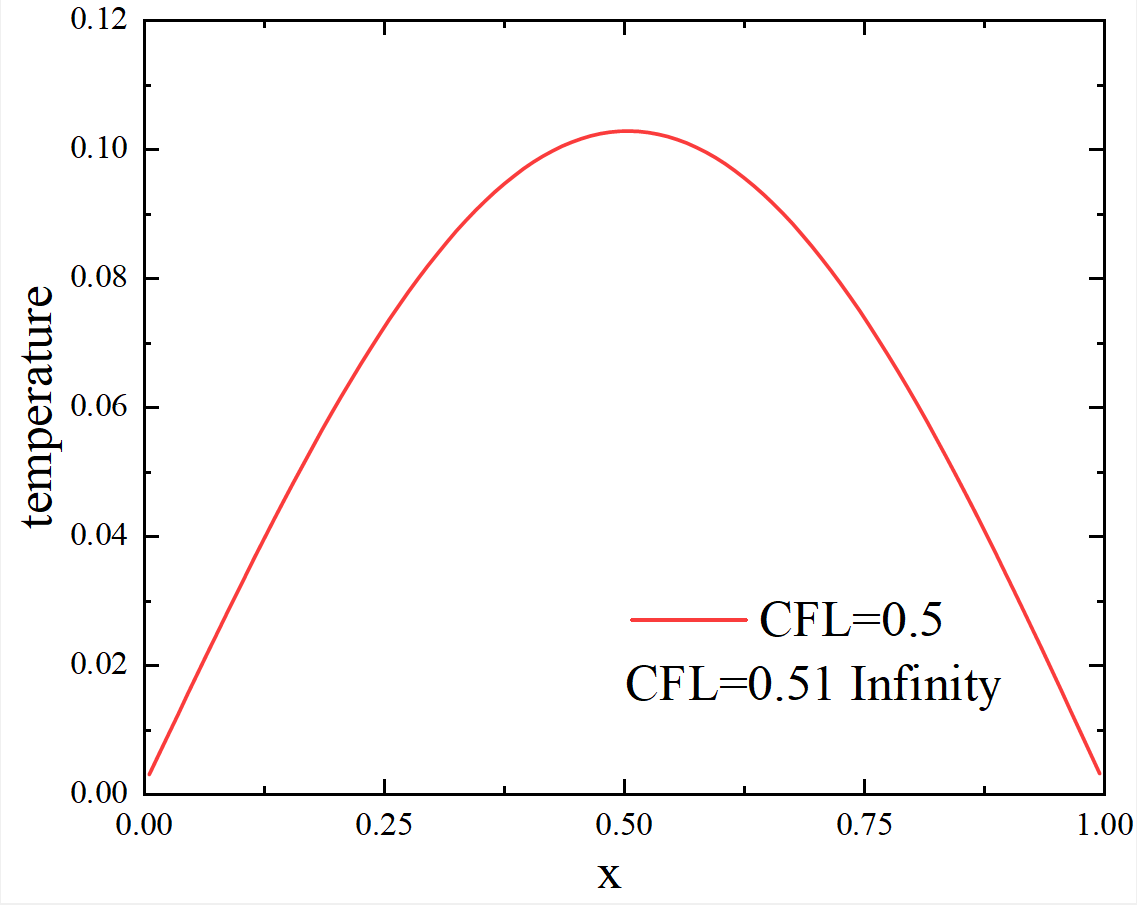
\includegraphics[width=0.7\linewidth]{screenshot003}
			\caption[]{不同CFL同一时刻的温度值对比}
			\label{fig:screenshot003}
		\end{figure}
		
		\subsection{误差分析}
		在该节中,首先从理论分析方程的误差阶数。不论是对于显式还是隐式格式,根据其泰勒展开式可以分析,其忽略的首项(称为截断误差)可以写为
		$$
		\frac{\Delta t}{2}\frac{\partial ^2u}{\partial t^2},\frac{(\Delta x)^2}{12}\frac{\partial ^4u}{\partial x^4}
		$$
		$$
		truncation \quad error=O(\Delta t,(\Delta x)^2)
		$$
		说明显式格式和隐式格式在时间上具有一阶精度,在空间上具有二阶精度。
		使用稳态解(即$\partial u /\partial t =0$)作为解析解计算误差$e$。当$\partial u /\partial t =0$时,原热传导方程化为:
		$$
		\frac{\partial^2 u}{\partial x^2}=-\frac{sin(l\pi x)}{\kappa}
		$$
		对其左右两式积分两次,得到
		$$
		u(x)=\frac{sin(l\pi x)}{(l\pi)^2\kappa}+C_1x+C_2
		$$
		其中$C_1,C_2$为待定常数。将边界条件代入,可以解得
		$$
		C_1=-\frac{sin(l\pi)}{(l\pi)^2\kappa},C_2=0
		$$
		故
		$$
		u(x)=\frac{sin(l\pi x)}{(l\pi)^2\kappa}-\frac{sin(l\pi)}{(l\pi)^2\kappa}x
		$$
		令$u_{exact}=u(x_j)$,定义误差为$e:=max_{1\leq j \leq n}|u_{exact,j}-u_{num,j}|$,则误差可以表达为与网格分辨率和时间步有关的函数$e \approx C_1\Delta x^{\alpha}+C_2\Delta t^{\beta}$。下面选取一个实例进行理论和代码的互验。本部分选取隐式方程试验(因为隐式解是无条件稳定的,可以自由调整网格分辨率和时间步的大小),选取的参数为$N=10,20,40,80,160,320,640,1280;\Delta t=1\times10^{-5};t_{end}=2.0$,而误差的阶数可以根据式$O=log_2(e_{\Delta x}/e_{\Delta x/2})$得到。数据如表1所示。可以看到,误差阶数普遍非常接近2,从而理论和代码成功实现了互验。
		\begin{table}[h]
			\centering
			\caption{不同精度网格的误差及阶数}\label{tab:aStrangeTable}%添加标题 设置标签
			\begin{tabular}{ccc}
				\toprule  %添加表格头部粗线
				网格分辨率N &最大误差e & 误差阶数 \\
				\midrule  %添加表格中横线
				
				10	& 0.021595 & -       \\
				20	& 0.011064 & 1.951826 \\
				40	& 0.005594 & 1.977833393 \\
				80	& 0.002813 & 1.988624245 \\
				160	& 0.001410 & 1.995035461 \\
				320	& 0.000706 & 1.997167139 \\
				640	& 0.000353 & 2 \\
				1280& 0.000177 & 1.994350282 \\
				
				\bottomrule %添加表格底部粗线
			\end{tabular}
		\end{table}
		
		
		\section{并行化测试}
		
		本章节将
		
\end{document}
